\section{Durchführung}
\label{sec:Durchführung}

Der Aufbau des Versuches ist in \autoref{fig:aufbau} dargestellt.
\begin{figure}
    \centering
    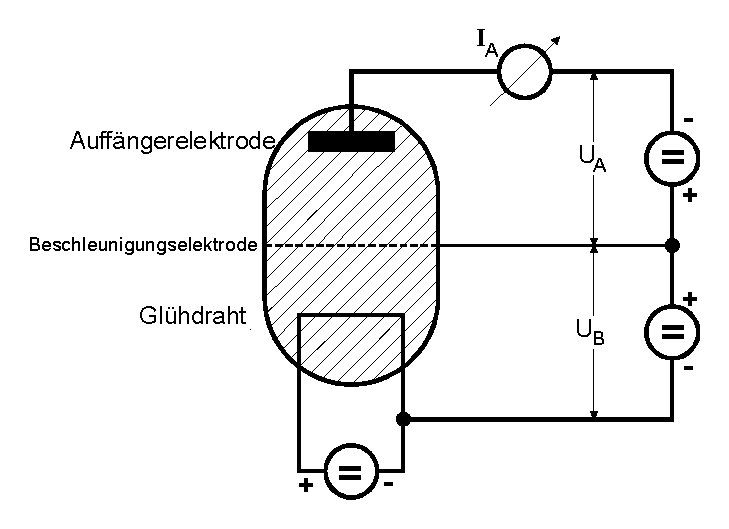
\includegraphics[width=0.7\linewidth]{pictures/aufbau.pdf}
    \caption{Ein Foto des Versuchsaufbaus \cite{v602}.}
    \label{fig:aufbau}
\end{figure}
Der Aufbau, im Wesentlichen bestehend aus einer Kupfer-Röntgenröhre, 
einem LiF-Kristall und einem Geiger-Müller-Zählrohr, ist an ein Computer angeschlossen.
Mithilfe des Programms \enquote{Measure} werden die notwendigen Einstellungen vorgenommen
und die Daten aufgenommen.


\subsection{Braggsche Bedingung}

Zur Überprüfung der Braggschen Bedingung wird das Geiger-Müller-Zählrohr
bei einem festen Kristall-Winkel von $\theta = \qty{14}{°}$ gedreht.
Dafür wird der Winkel des Zählrohrs $\alpha_\text{GM}$ im Intervall von $\qty{26}{°}$ bis $\qty{30}{°}$ bei einer Integrationszeit von 
$\increment t = \qty{5}{s}$ in Schritten von $\increment \alpha = \qty{0.1}{°}$ variiert. 


\subsection{Emissionsspektrum}

Für die Untersuchung des Emissionsspektrums der Röntgenstrahlung wird im Programm
die Option 2:1 Koppelmodus eingestellt, 
damit das Geiger-Müller-Zählrohr stets im doppelten Winkel des Kristalls steht,
sodass die größtmögliche Intensität der entsprechenden Wellenlänge gemessen wird.
Bei einer Integrationszeit von $\increment t = \qty{5}{s}$ wird im Winkelintervall 
$\theta \in [\qty{4}{°}, \qty{26}{°}]$ in Schritten von $\increment \theta = \qty{0.2}{°}$
das Emissionsspektrum gemessen.
Nachdem die charakteristischen Peaks der $K_\alpha$- und $K_\beta$-Linie festgestellt wurden,
werden diese in einem Detailspektrum für $\theta \in [\qty{18}{°}, \qty{24}{°}]$ bei einer Schrittweite von $\increment \theta = \qty{0.1}{°}$ gemessen.


\subsection{Absorptionsspektrum}

Die Messung des Absorptionsspektrum erfolgt hierbei durch verschiedene Absorberstoffe, 
welche auf das Geiger-Müller-Zählrohr aufgesetzt werden.
Die Literaturwerte der K-Kanten dieser Stoffe sind in \autoref{tab:literatur} dargestellt.
Bei gleichem Winkelschritt wird für fünf verschiedene Absorber bei einer Integrationszeit von $\increment t = \qty{20}{s}$ gemessen.
Die hier verwendeten Stoffe sind Zink, Gallium, Brom, Strontium und Zirkonium.